% !TEX root = micro_Lie_theory.tex

\newcommand{\dx}{{\delta\bfx}}

\section{基于地标的定位与建图}
\label{sec:SLAM}

我们提供了三个机器人定位和建图理论的应用实例。 
第一个是基于Kalman滤波的地标定位方法。
第二个是基于图的平滑方法,用于同时定位和建图。
第三个增加了传感器自校正。
它们基于一个公共设置,解释如下。

我们考虑一个在平面上的机器人
(对于三维情况,参见 \secRef{sec:demos_3D})
周围有少量准时的地标或信标(\emph{beacons})。 
机器人以轴向速度和角速度的形式接收控制动作,并且能够测量信标相对于其自身参考坐标系的位置。


机器人姿态在 $\SE(2)$ 中 (\appRef{sec:SE2}) ,并且信标位置在 $\bbR^2$ 中 (\appRef{sec:Tn}),
%
\begin{align*}
\cX &= 
\begin{bmatrix}
\bfR & \bft \\ \bf0 & 1
\end{bmatrix}\in\SE(2)
~,
&
\bfb_k &= \begin{bmatrix}
x_k \\ y_k
\end{bmatrix}\in\bbR^2
~.
\end{align*}

控制信号 $\bfu$ 是 $\se(2)$ 中的一个扭曲,包括纵向速度 $v$ 和角速度 $\omega$,没有横向速度分量,在采样时间 $\dt$ 内积分。
该控制已被加性高斯噪声 $\bfw\sim\cN(\bf0,\bfW)$ 损坏。
此噪声可能视为车轮横向打滑 $u_s$ ,数值为 $\sigma_s\ne0$,
%
\begin{align}
\bfu &
= \begin{bmatrix} u_v \\ u_s \\ u_\omega \end{bmatrix} 
= \begin{bmatrix} v\,\dt \\ 0 \\ \omega\,\dt \end{bmatrix}+\bfw  
&&\in\se(2)
\\
\bfW &= \begin{bmatrix}
\sigma_v^2\dt &0&0 \\ 0&\sigma_s^2\dt&0 \\ 0&0&\sigma_w^2\dt
\end{bmatrix} &&\in\bbR^{3\times3}.
\end{align}
%
当一个控制 $\bfu_j$ 在时间 $j$ 到达时,机器人的姿态将更新为方程 \eqRef{equ:int_recursive},
%
\begin{align}\label{equ:motion}
\cX_j &= \cX_i \op \bfu_j \te \cX_i \Exp(\bfu_j)
~.
\end{align}


%
地标测量是有范围和承载类型的,尽管为了简单起见,它们被放在笛卡尔形式中。
它们的噪声 $\bfn\sim\cN({\bf0},\bfN)$ 是零均值高斯分布,
%
\begin{align}\label{equ:meas_beacon}
\bfy_k &= \cX\inv\cdot\bfb_k + \bfn = \bfR\tr(\bfb_k-\bft) + \bfn	&&\in \bbR^2
\\
\bfN &= \begin{bmatrix}
\sigma_x^2 &0 \\ 0& \sigma_y^2
\end{bmatrix}										&&\in\bbR^{2\times2}
~,
\end{align}
%
其中我们注意到刚体运动作用 $\cX\inv\cdot\bfb_k$ (参见 \appRef{sec:SE2})。




%%%%%%%%%%%%%%%%%%%%%%%%%%%%%%%%%%%%%%%%%%%%%%%%%%%%%%%%%%%%%%%%
\subsection{基于流形的误差状态Kalman滤波定位}
\label{sec:loc_ESKF}

我们最初考虑信标 $\bfb_k$ 位于已知位置。 
我们将要估计的姿态定义为 $\hat\cX\in\SE(2)$。
估计误差 $\dx$ 及其协方差 $\bfP$ 在 $\hat\cX$ 处切空间中用方程 \eqssRef{equ:uncertainty,equ:cov} 表示,
%
\begin{align}\label{equ:loc_Gaussian}
\dx &\te \cX\ominus\hat\cX && \in\bbR^3
\\
\bfP &\te \bbE[(\cX\ominus\hat\cX)(\cX\ominus\hat\cX)\tr]&& \in\bbR^{3\times3}
~.
\end{align}
%
在机器人的每一个运动中,我们应用ESKF预测,
%
\begin{align}
\hat\cX_j &= \hat\cX_i\op\bfu_j \label{equ:loc_ekf_pred}
\\
\bfP_j &= \bfF\,\bfP_i\,\bfF\tr + \bfG\,\bfW_j\,\bfG\tr
~,
\end{align}
%
用 \appRef{sec:SE2} 中的块计算 Jacobians 矩阵,
%
\begin{align*}
\bfF &\te \mjac{\cX_j}{\cX_i} = \mjac{\hat\cX_i\op\bfu_j}{\hat\cX_i} 
= \Ad{\Exp(\bfu_j)}\inv
\\
\bfG &\te \mjac{\cX_j}{\bfu_j} = \mjac{\hat\cX_i\op\bfu_j}{\bfu_j} = \mjac{}{r}(\bfu_j)
~.
\end{align*}
%
在每个信标测量 $\bfy_k$ 时,我们应用ESKF校正,
%
\begin{align}
\textrm{Innovation}&:&\bfz &= \bfy_k - \hat\cX\inv\cdot\bfb_k \notag\\
\textrm{Innovation cov.}&:&\bfZ &= \bfH\,\bfP\,\bfH\tr+\bfN \notag\\
\textrm{Kalman gain}&:&\bfK &= \bfP\,\bfH\tr\,\bfZ\inv \notag\\
\textrm{Observed error}&:&\dx &= \bfK\bfz \notag\\
\textrm{State update}&:&\hat\cX &\gets \hat\cX \oplus \dx \label{equ:loc_ekf_corr}\\
\textrm{Cov. update}&:&\bfP &\gets \bfP - \bfK\,\bfZ\,\bfK\tr
~,
\end{align}
%
用 \appRef{sec:SE2} 中的块计算 Jacobians 矩阵,
\begin{align*}
\bfH 
&\te \mjac{\cX\inv\cdot\bfb_k}{\cX}= \mjac{\cX\inv\cdot\bfb_k}{\cX\inv}\,\mjac{\cX\inv}{\cX} 
\notag\\
&= 
\begin{bmatrix}\bfR\tr & \bfR\tr\hatx{1}\bfb_k\end{bmatrix}
\begin{bmatrix}
-\bfR & \hatx{1}\bft \\ \bf0 & -1
\end{bmatrix}
\notag\\
&=
-\begin{bmatrix}\bfI & \bfR\tr\hatx{1}(\bfb_k-\bft)\end{bmatrix}
~.
\end{align*}

注意,相对于常规EKF的唯一更改在方程 \eqRef{equ:loc_ekf_pred} 和方程 \eqRef{equ:loc_ekf_corr},其中常规的 $+$ 被用 $\op$ 替换。
相反地,Jacobian矩阵都用Lie理论计算(参见 \appRef{sec:SE2})。
有趣的是,它们的用法与标准EKF中的用法相同 --- 例如,参见Kalman增益方程,即标准的 $\bfK = \bfP\bfH\tr(\bfH\bfP\bfH\tr+\bfN)\inv$ 。


%%%%%%%%%%%%%%%%%%%%%%%%%%%%%%%%%%%%%%%%%%%%%%%%%%%%%%%%%%%%%%%%
\subsection{基于图优化的平滑和建图}
\label{sec:SAM}

我们现在考虑平滑和映射(SAM)问题,其中要估计的变量是信标的位置和机器人的轨迹。
选择的解算器是一个基于图的迭代最小二乘优化器。
为简单起见,我们假设轨迹由三个机器人姿态 $\{\cX_1\cdots\cX_3\}$ ,一个有三个信标 $\{\bfb_4\cdots\bfb_6\}$ 的世界组成。
问题状态是组合的
%
\begin{align}\label{equ:SAM_state}
\cX &= \langle
\cX_1 , \cX_2 , \cX_3 , \bfb_4 , \bfb_5 , \bfb_6
\rangle, \quad \cX_i\in\SE(2),\quad\bfb_k\in\bbR^2.
\end{align}
%
结果因子图 \cite{DELLAERT-IJRR-06} 如 \figRef{fig:graph-SLAM} 所示。
每一个先验或测量值在图中贡献一个因子。
从姿态 $i$ 到 $j$ 的运动测量值来自方程 \eqRef{equ:motion},
当信标 $k$ 从姿态 $i$ 的测量时响应方程 \eqRef{equ:meas_beacon},
%
\begin{figure}
\centering
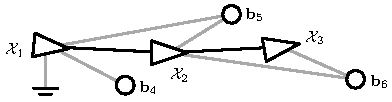
\includegraphics{figures/SAM}
\caption{具有3个姿态和3个信标的SAM因子图。
每一个测量值在图中贡献一个因子。
这里有2个运动因子(黑色)和5个信标因子(灰色)。
在 $\cX_1$ 上的先验因子提供全局可观测性。}
\label{fig:graph-SLAM}
\end{figure}
%
%
\begin{align}
\bfu_{ij} &= \cX_j\ominus\cX_i + \bfw_{ij} = \Log(\cX_i\inv\cX_j) + \bfw_{ij} \label{equ:meas_motion} \\
\bfy_{ik} &= \cX_i\inv\cdot\bfb_k + \bfn_{ik}
~.
\end{align}
%
每一个因子都有一个信息矩阵, $\bfOmega_{1} \te \bfW_{1}\inv$, $\bfOmega_{ij} \te \bfW_{ij}\inv$ 和 $\bfOmega_{ik} \te \bfN_{ik}\inv$ 。
%
期望残差(residual)是,
%
\begin{align}
\textrm{prior residual}&:&\bfr_{1}(\cX) &= \bfOmega_{1}^{\top/2}(\cX_1 \om \hat\cX_1)
\notag
\\
\textrm{motion residual}&:&\bfr_{ij}(\cX) &= \bfOmega_{ij}^{\top/2}(\bfu_{ij} - (\hat\cX_j\ominus\hat\cX_i))
\notag
\\
\textrm{beacon residual}&:&\bfr_{ik}(\cX) &= \bfOmega_{ik}^{\top/2}(\bfy_{ik} - \hat\cX_i\inv\cdot\hat\bfb_k)
\notag
~.
\end{align}
%
最佳更新步骤 $\dx$ 源自于最小化
%
\begin{align}\label{equ:SAM_problem}
\dx^* = \argmin_{\dx} \sum_{p\in\cP} \bfr_p(\cX\dplus\dx)\tr\bfr_p(\cX\dplus\dx)
\end{align}
%
其中 $\cP=\{1,12,23,14,15,25,26,36\}$ 是每一个测量的节点对的集合 (参见 \figRef{fig:graph-SLAM}) 。
这个问题迭代求解如下。
总和方程 \eqRef{equ:SAM_problem} 中的每一个残差跟随方程 \eqRef{equ:lin_approx_composite} 被线性化为 $\bfr_p(\cX\dplus\dx)\approx\bfr_p(\cX)\dplus\mjac{\bfr_p}{\cX}\dx$ ,其中 $\mjac{\bfr_p}{\cX}$ 是稀疏Jacobian矩阵。
这些Jacobian矩阵的非零块,即 $\mjac{\bfr_{1}}{\cX_1}$, $\mjac{\bfr_{ij}}{\cX_i}$, $\mjac{\bfr_{ij}}{\cX_j}$, $\mjac{\bfr_{ik}}{\cX_i}$ 和 $\mjac{\bfr_{ik}}{\bfb_k}$,可以按照 \secRef{sec:loc_ESKF} 中的方法轻松计算,并注意到根据定义 $\mjac{f(\cX\op\dx)}{\dx}|_{\dx=0}=\mjac{f(\cX\op\dx)}{\cX}|_{\dx=0}=\mjac{f(\cX)}{\cX}$。
%
建立总的Jacobian矩阵和残差向量,
%
\begin{align}\label{equ:SAM_problem_lin}
\bfJ &= \begin{bmatrix}
\mjac{\bfr_{1}}{\cX_1} & \bf0 & \bf0 & \bf0 & \bf0 & \bf0 \\ 
\mjac{\bfr_{12}}{\cX_1} & \mjac{\bfr_{12}}{\cX_2} & \bf0 & \bf0 & \bf0 & \bf0 \\ 
\bf0 & \mjac{\bfr_{23}}{\cX_2} & \mjac{\bfr_{23}}{\cX_3} & \bf0 & \bf0 & \bf0 \\ 
\mjac{\bfr_{14}}{\cX_1} & \bf0 & \bf0 & \mjac{\bfr_{14}}{\bfb_4} & \bf0 & \bf0 \\ 
\mjac{\bfr_{15}}{\cX_1} & \bf0 & \bf0 & \bf0 & \mjac{\bfr_{15}}{\bfb_5} & \bf0 \\ 
\bf0 & \mjac{\bfr_{25}}{\cX_2} & \bf0 & \bf0 & \mjac{\bfr_{25}}{\bfb_5} & \bf0 \\ 
\bf0 & \mjac{\bfr_{26}}{\cX_2} & \bf0 & \bf0 & \bf0 & \mjac{\bfr_{26}}{\bfb_6} \\ 
\bf0 & \bf0 & \mjac{\bfr_{36}}{\cX_3} & \bf0 & \bf0 & \mjac{\bfr_{36}}{\bfb_6} 
\end{bmatrix}
&
\bfr &= \begin{bmatrix}
\bfr_{1} \\
\bfr_{12} \\
\bfr_{23} \\
\bfr_{14} \\
\bfr_{15} \\
\bfr_{25} \\
\bfr_{26} \\
\bfr_{36}
\end{bmatrix}
\end{align}
%
线性化的方程 \eqRef{equ:SAM_problem} 现在转换为 \cite{DELLAERT-IJRR-06} 最小化
%
\begin{align}
\dx^* 
 &= \argmin_\dx \norm{\bfr+\bfJ\dx}^2
.
\end{align}
%
这通过使用 $\bfJ$ 的伪逆的最小二乘法来解决 (对于大型问题,需要 QR \cite{DELLAERT-IJRR-06,KAESS-11-ISAM2} 或 Cholesky \cite{KUMMERLE-11-G2O,ILA-17_SLAM++} 的因式分解),
%
\begin{align}
\dx^* &= -(\bfJ\tr\bfJ)\inv\bfJ\tr\bfr \label{equ:SAM_opt_step}
~,
\intertext{产生用于更新状态的最佳步骤 $\dx^*$ ,}
\cX &\gets \cX \dplus \dx^* \label{equ:SAM_update}
~.
\end{align}
%
这个过程被迭代直到收敛。

我们在此强调在方程 \eqRef{equ:SAM_state} 中组合符号的使用,它允许按块定义Jacobian矩阵方程 \eqRef{equ:SAM_problem_lin} 和更新方程 \eqRef{equ:SAM_update} 。我们还注意到 $\SE(2)$ 流形在运动和测量模型中的使用,正如我们在 \secRef{sec:loc_ESKF} 中的ESKF案例中所做的那样。


%%%%%%%%%%%%%%%%%%%%%%%%%%%%%%%%%%%%%%%%%%%%%%%%%%%%%%%%%%%%%%%%
\subsection{自校正平滑和建图}

我们考虑与上述问题相同的问题,但运动传感器受到未知校正偏差 $\bfc=(c_v,c_\omega)\tr$ 的影响,
 所以控制现在是 $
\tilde\bfu 
=
(v\dt + c_v ,~
0 ,~
\omega \dt + c_\omega)\tr + \bfw
$.
%
我们定义偏差校正函数 $c()$ ,
%
\begin{align}\label{equ:bias}
\bfu &= c\,(\tilde\bfu, \bfc) \te \begin{bmatrix}
\tilde u_v - c_v \\
\tilde u_s \\
\tilde u_\omega - c_\omega
\end{bmatrix} \quad \in \bbR^3\cong\se(2)
~.
\end{align}
%
状态组合用未知的 $\bfc$ 扩充,
%
\begin{align*}
\cX &= \langle
\bfc, \cX_1 , \cX_2 , \cX_3 , \bfb_4 , \bfb_5 , \bfb_6
\rangle
~, 
\\
\bfc&\in\bbR^2,\qquad\cX_i\in\SE(2),\qquad\bfb_k\in\bbR^2
~,
\end{align*}
%
并且运动残差变为
%
\begin{align*}
\bfr_{ij}(\cX) &= \bfOmega_{ij}^{\top/2}\big(c\,(\tilde\bfu_{ij} , \bfc) - (\hat\cX_j\ominus\hat\cX_i)\big)
~.
\end{align*}
%
步骤如上面 \secRef{sec:SAM} 一样,并且总Jacobian矩阵在左边加了一列,
%
\begin{align*}
\bfJ &= \begin{bmatrix}
\bf0 & \mjac{\bfr_{1}}{\cX_1} & \bf0 & \bf0 & \bf0 & \bf0 & \bf0 \\ 
\mjac{\bfr_{12}}{\bfc} & \mjac{\bfr_{12}}{\cX_1} & \mjac{\bfr_{12}}{\cX_2} & \bf0 & \bf0 & \bf0 & \bf0 \\ 
\mjac{\bfr_{23}}{\bfc} & \bf0 & \mjac{\bfr_{23}}{\cX_2} & \mjac{\bfr_{23}}{\cX_3} & \bf0 & \bf0 & \bf0 \\ 
\bf0 & \mjac{\bfr_{14}}{\cX_1} & \bf0 & \bf0 & \mjac{\bfr_{14}}{\bfb_4} & \bf0 & \bf0 \\ 
\bf0 & \mjac{\bfr_{15}}{\cX_1} & \bf0 & \bf0 & \bf0 & \mjac{\bfr_{15}}{\bfb_5} & \bf0 \\ 
\bf0 & \bf0 & \mjac{\bfr_{25}}{\cX_2} & \bf0 & \bf0 & \mjac{\bfr_{25}}{\bfb_5} & \bf0 \\ 
\bf0 & \bf0 & \mjac{\bfr_{26}}{\cX_2} & \bf0 & \bf0 & \bf0 & \mjac{\bfr_{26}}{\bfb_6} \\ 
\bf0 & \bf0 & \bf0 & \mjac{\bfr_{36}}{\cX_3} & \bf0 & \bf0 & \mjac{\bfr_{36}}{\bfb_6} 
\end{bmatrix}
~,
\end{align*}
%
其中 $\mjac{\bfr_{ij}}{\bfc} = \bfOmega_{ij}^{\top/2}\mjac{c(\bfu_{ij} , \bfc)}{\bfc}$,其中 $\mjac{c(\bfu_{ij} , \bfc)}{\bfc}$ 是方程 \eqRef{equ:bias} 的 $3\times 2$ 的Jacobian矩阵。
最优解用方程 \eqssRef{equ:SAM_opt_step,equ:SAM_update} 获得。
得到的最优状态 $\cX$ 包括 $\bfc$ 的最优估计,即传感器偏差的自校正。

\subsection{3D实现}
\label{sec:demos_3D}

把上面所有的例子都放到3D上是非常容易的。
在正确的空间中定义所有变量就足够了:
$\cX\in\SE(3)$ 和 $\bfu\in\bbR^6\cong\se(3)$ (\appRef{sec:SE3}), 和 $\{\bfb_k,\bfy\}\in\bbR^3$ (\appRef{sec:Tn})。
Jacobian矩阵和协方差矩阵将遵循适当的大小。
%
这里有趣的地方在于认识到算法中的所有数学,即从方程 \eqRef{equ:loc_Gaussian} 出发,对于2D和3D来说是完全一样的:Lie理论提供的抽象层次使这成为可能。

